% Source for the figure of Mailbox on MeshChannels (sec. 25.13): three
% workers, the outbox of the worker 0 for the worker 1, the queue of the
% pair (0, 1) of the mesh and the shared counter C, before and after the
% push of a batch of three messages. Build: make figures (in ../build).
\documentclass[border=4pt]{standalone}
\usepackage[T1]{fontenc}
\usepackage{lmodern}
\usepackage{amsmath,amssymb}
\usepackage{tikz}
\usepackage{lamalunga}
% tikz-ads.tex: the TikZ styles shared by the figures of the memory of the
% manual, \input by each standalone figure: a cell of a vector (cell), the
% cell that an operation touches (touched), a free cell (free), a node of a
% linked structure (node), the labels of indices (index) and of variables
% (var), a pointer (ptr), and \cells and \indices to draw a row of cells.
\usetikzlibrary{arrows.meta,positioning,calc,fit,shapes.multipart}
\definecolor{adsTouched}{RGB}{214,196,236}
\definecolor{adsFree}{RGB}{236,236,236}
\tikzset{
  ads/.style={>={Stealth[length=2mm]},font=\small,
              every node/.append style={inner sep=0pt}},
  cell/.style={draw,minimum width=7mm,minimum height=7mm,
               font=\small\ttfamily,outer sep=0pt},
  touched/.style={cell,fill=adsTouched},
  free/.style={cell,fill=adsFree,text=black!45},
  node/.style={draw,rounded corners=1pt,minimum width=8mm,
               minimum height=6mm,font=\small\ttfamily},
  index/.style={font=\scriptsize\ttfamily,text=black!60},
  var/.style={font=\small\itshape},
  ptr/.style={->,thick}
}
% \cells{name}{x,y}{list}: a row of cells, the first at (x,y), named
% name-0, name-1, ...; each item is text/style, the style one of cell,
% touched and free (e.g., {a/cell,e/touched,/free})
\newcommand{\cells}[3]{%
  \foreach \v/\s [count=\i from 0] in {#3}
    \node[\s] (#1-\i) at ($(#2)+(\i*7mm,0)$) {\v};}
% \indices{name}{n}: the indices 0 .. n-1 under the cells of name
\newcommand{\indices}[2]{%
  \foreach \i in {0,...,\numexpr#2-1\relax}
    \node[index,below=1.2mm of #1-\i] {\i};}

\begin{document}
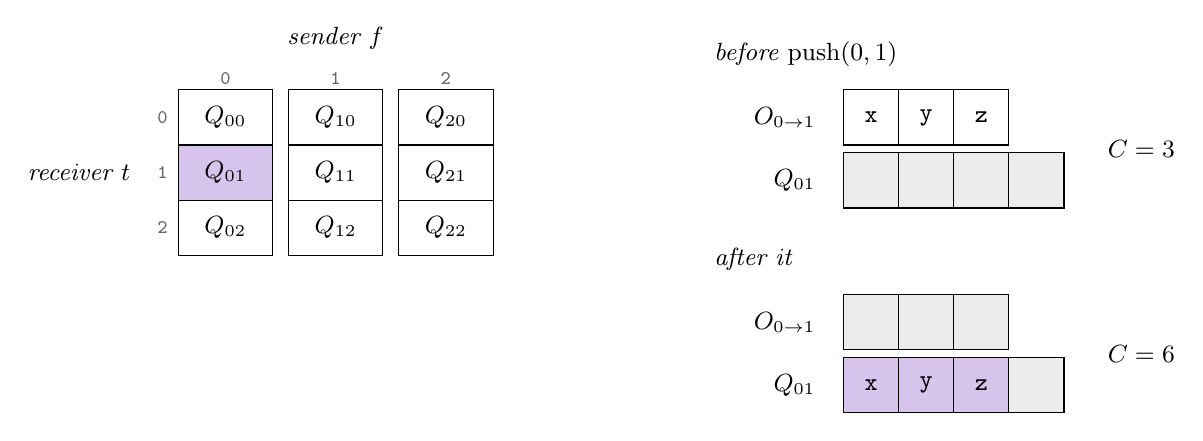
\begin{tikzpicture}[ads]
  % the mesh of p = 3 workers: the queue Q_{f,t} in the row t, column f
  \node[var] at (14mm,10mm) {sender $f$};
  \foreach \f in {0,1,2} \node[index] at (\f*14mm,5mm) {\f};
  \node[var,anchor=east] at (-12mm,-7mm) {receiver $t$};
  \foreach \t in {0,1,2} {
    \node[index] at (-8mm,-\t*7mm) {\t};
    \foreach \f in {0,1,2}
      \node[cell,minimum width=12mm,font=\small] (q\f\t) at (\f*14mm,-\t*7mm)
        {$Q_{\f\t}$};
  }
  \node[cell,minimum width=12mm,font=\small,fill=adsTouched] at (0,-7mm)
    {$Q_{01}$};
  % before and after the push
  \begin{scope}[xshift=62mm]
  \node[var,anchor=west] at (0,8mm) {before $\mathrm{push}( 0 , 1 )$};
  \node[var,anchor=east] at (13mm,0) {$O_{0 \to 1}$};
  \cells{a}{20mm,0}{x/cell,y/cell,z/cell}
  \node[var,anchor=east] at (13mm,-8mm) {$Q_{01}$};
  \cells{b}{20mm,-8mm}{/free,/free,/free,/free}
  \node[var,anchor=west] at (50mm,-4mm) {$C = 3$};
  \node[var,anchor=west] at (0,-18mm) {after it};
  \node[var,anchor=east] at (13mm,-26mm) {$O_{0 \to 1}$};
  \cells{c}{20mm,-26mm}{/free,/free,/free}
  \node[var,anchor=east] at (13mm,-34mm) {$Q_{01}$};
  \cells{d}{20mm,-34mm}{x/touched,y/touched,z/touched,/free}
  \node[var,anchor=west] at (50mm,-30mm) {$C = 6$};
  \end{scope}
\end{tikzpicture}
\end{document}
